\chapter{Implementación}
\label{chap:implementación}

\lettrine{N}{este} capítulo explicase o proceso de implementación, as decisións importantes durante este, os problemas atopados e as súas solucións.

\section{Estrutura do proxecto}
Na seguinte figura~\ref{fig:estrutura_xeral} amósase a estrutura xeral do proxecto e a súa xerarquía de cartafois. Debido a que o proxecto conta con un backend e un frontend existen dúas partes na estrutura ben diferenciadas, primeiro descríbese a estrutura do backend e a continuación a do frontend.\medbreak

A estrutura principal do backend é similar a dos proxectos \textit{Django}, conta cun proxecto chamado \textit{Wikebackend} e dúas aplicacións, unha chamada \textit{users} que é a encargada da xestión dos usuarios e a outra \textit{api} que é a que xestiona as peticións recibidas e as enviadas a API de Spotify. 

\begin{figure}[h!]
  \centering
  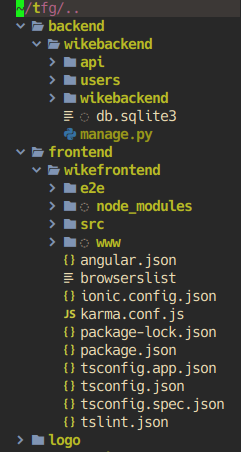
\includegraphics[width=0.3\textwidth]{imaxes/estrutura_xeral.png}
  \caption{Estrutura do proxecto}
  \label{fig:estrutura_xeral}
\end{figure}

\begin{itemize}
	\item \textbf{Wikebackend}\smallbreak
		Garda os arquivos de configuración de Django, entre eles as opcións en \textit{settings.py}. Neste arquivo se almacenan aspectos básicos da configuración, coma son as apps utilizadas, o método de autenticación, o tipo de base de datos, a linguaxe, configuración da zona horaria\dots~ Nesta parte da estrutura tamén se almacena a redirección de urls principal no arquivo \textit{urls.py} este redirixe as peticións que recibe aos ficheiros axeitados. 
	\item \textbf{Api}\smallbreak
		Trátase da parte principal do proxecto, é a parte encargada de gran parte da lóxica de este, encárgase de xestionar as peticións recibidas e devolver as respostas axeitadas. Tamén contén as peticións necesarias para a iteración coa API de Spotify.
	\item \textbf{Users}\smallbreak
		É a aplicación que xestiona os usuarios, contén as modificacións para a adaptación do modelo de usuarios ao proxecto e as funcións que teñen que ver con estes.
\end{itemize}

\begin{figure}[h!]
  \centering
  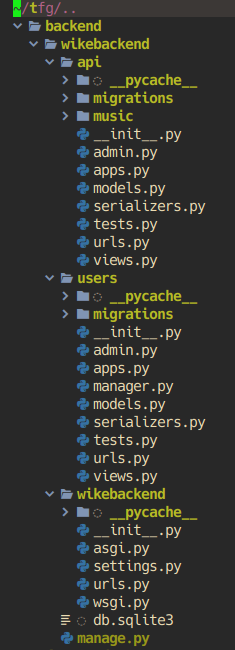
\includegraphics[width=0.3\textwidth]{imaxes/estrutura_backend.png}
  \caption{Estrutura do backend}
  \label{fig:estrutura_backend}
\end{figure}

Respecto ao frontend a estrutura segue a distribución xeral dos proxectos en \textit{Ionic} dentro do cartafol \textit{src} atopamos a todo o código do proxecto, describese a estrutura a continuación.

\begin{itemize}
	\item \textbf{App}\smallbreak
		Contén toda a lóxica do frontend, ao igual que no backend esta é unha app dentro do proxecto que conta con características únicas dentro deste. Ademais de almacenar as páxinas, tamén contén os servizos, os modelos e os compoñentes utilizados.
	\item \textbf{Assets}\smallbreak
		Neste cartafol gárdanse todos os recursos, tales coma poderían ser clips de son, vídeos ou imaxes, que é o caso do proxecto, deste xeito facilitase a orde e o acceso a este tipo de recursos.
	\item \textbf{Environments}\smallbreak
		Ao igual que moitas outras ferramentas de desenvolvemento, Ionic contén configuracións específicas para o traballo en produción e en desenvolvemento, o que facilita o cambio dun entorno a outro cando se queren facer modificacións, estes arquivos gárdanse no cartafol environments.
	\item \textbf{Theme}\smallbreak 
		Almacea as variables correspondentes a folla de estilo, garda as cores principais para axeitar todo o proxecto a un tema en concreto e non ter que introducir as cores por separado en canda sexan necesarias.
\end{itemize}

\begin{figure}[h!]
  \centering
  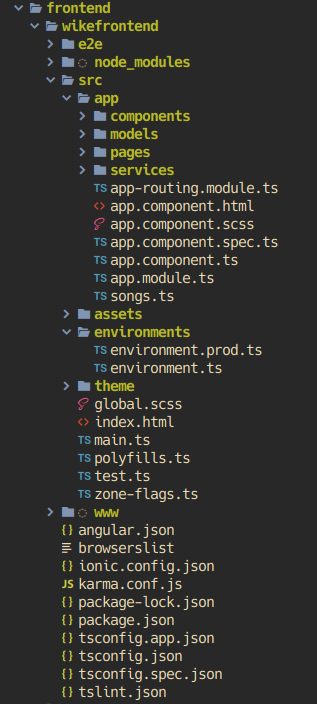
\includegraphics[width=0.3\textwidth]{imaxes/estrutura_frontend.png}
  \caption{Estrutura do frontend}
  \label{fig:estrutura_frontend}
\end{figure}

A continuación descríbese en profundidade as partes mais extensas que son a aplicación \textbf{api} no backend e a \textbf{app} no frontend:

\textbf{Api} é parte do backend, consta dos arquivos xerais dunha aplicación Django, \textit{urls.py} e o arquivo encargado de xestionar as peticións e executar as funcións de \textit{views.py}. En \textit{models.py} como o seu nome indica defínense os modelos, neste caso as sesións, as cancións que se están a reproducir e as da cola, para facilitar o almacenamento de datos nos modelos utilízanse os serializadores, definidos no arquivo \textit{serializers.py}. Tamén conta cun ficheiro tan só para as peticións a api de Spotify chamado \textit{spotify.py} este é utilizado nas funcións das vistas.

\textbf{App} forma parte do frontend, e como xa vimos contén a maior parte do código de este, está formado principalmente polas páxinas web as que os usuarios terán acceso, pódense ver na sección~\ref{sec:paxinas_front}, estas contan cos seus módulos e as súas propias follas de estilos.\smallbreak
Para o correcto funcionamento das páxinas son necesarios os servizos, incluídos tamén neste apartado da estrutura, son os principais encargados de realizar as peticións ao backend, están divididos entre os xerais de api, autenticación e o interceptor, encargado de engadir as cabeceiras para o correcto funcionamento dos \acrshort{JWT}.\smallbreak
Os compoñentes tamén forman parte de este apartado, son bloques que conteñen funcionalidades específicas, neste caso son utilizados para amosar información en ventás emerxentes é o caso para os resultados das procuras ou a obtención do token de autenticación de Spotify.\smallbreak
Por último tamén se inclúen pequenos modelos utilizados para a transferencia de información, deste xeito dita información pódese xestionar como un bloque, neste caso son utilizados para a autenticación dos usuarios, o almacenamento dos tokens e as cancións.

\section{Seguridade}
Aínda que a aplicación non almacena datos sensibles, xa que o mais relevante é o token de autenticación de Spotify, foi necesario o desenvolvemento dun método seguro para a transferencia de información entre o backend e o frontend. Deste modo evítase que usuarios non rexistrados accedan a aplicación e especialmente conséguese que o usuario administrador teña a posibilidade de acceder a mais opcións sen que accedan a estas o resto de usuarios. A continuación descríbese o proceso de securizar a aplicación xa que conta con diferentes casos e realizouse en diferentes tempos do desenvolvemento.\smallbreak 
En calquera comunicación entre un backend e un frontend existe un intercambio de peticións \acrshort{HTTP}, cando son realizadas a un dominio, ou porto, diferente ao que pertence a aplicación que está realizando a petición, os navegadores a rexeitan por motivos de seguridade. Debido a isto é necesario utilizar cabeceiras \acrlong{CORS},~\footnote{Intercambio de Recursos de Orixe Cruzado.} o seu obxectivo é engadir as cabeceiras HTTP o conxunto de orixes que teñen permiso para ler a información usando o explorador web, deste xeito compróbase que a petición é lexitima e non se está intentando acceder a dominios non coñecidos. Para a modificación das cabeceiras é necesario incluír no middleware de Django a app chamada \textit{corsheaders}~\cite{corsHeaders} que se encarga de facer as modificacións necesarias.\smallbreak
Para comprobar a autenticidade do servidor utilizamos CORS, en cambio para autenticidade dos usuarios é necesario utilizar algún método, preferiblemente que fose o menos intrusivo posible, para isto estudáronse diferentes metodoloxías e posibilidades baseándose nas posibilidades de tanto Django coma Ionic. En Django existen varios métodos preestablecidos para realizar a autenticación:
\begin{itemize}
	\item \textbf{Autenticación básica:} envía tanto o usuario como o contrasinal en texto plano.
	\item \textbf{Autenticación de sesión:} utiliza o propio backend de Django para manter as sesións.
	\item \textbf{Autenticación remota:} permite o uso dun servidor externo que é o encargado de realizar a autenticación.
	\item \textbf{Autenticación con tokens:} utiliza tokens de acceso e refresco para comprobar que as peticións son lexítimas.
	\item \textbf{Autenticación personalizada:} permite crear un tipo de autenticación propio axeitado para as necesidades exactas.
\end{itemize}
Tamén existe a opción de utilizar paquetes de terceiros con diferentes métodos de autenticación coma OAuth ou \acrshort{JWT}~\cite{djangoAuth}.\smallbreak
Estudáronse estes métodos e concluíuse que o mais axeitado sería o uso de sesións ou tokens. A autenticación por sesións non sería axeitada para a comunicación entre o backend e o frontend debido a que está pensada para o seu uso en clientes \textit{AJAX} que funcionan no mesmo contexto que a propia páxina web, polo tanto a elección final é utilizar un sistema de autenticación por tokens. Novamente existen dúas eleccións, o uso de \textbf{OAuth} ou \textbf{\acrshort{JWT}}. Aínda que a autenticación con OAuth podería ser moi axeitada declinouse debido a intención de simplificar o máximo, aínda que cabe destacar que nun futuro sería unha opción a contemplar xa que permitiría unificar as contas de usuarios entre sesións.\smallbreak
Finalmente a opción elixida foi o uso de \acrshort{JWT}, existen paquetes de terceiros para facilitar o manexo de \acrshort{JWT} con Django, o mais coñecido é \textit{SimpleJWT}~\cite{simpleJWT} que xera un token de acceso con unha caducidade de 5 minutos e un de refresco con caducidade para 24 horas. No caso de Ionic foi necesaria a creación dun \textit{interceptor} que é o encargado tanto de engadir o token as cabeceiras nas peticións, coma de facer a comprobación de se é necesario renovar o token de acceso cada vez que recibe unha nova petición.\smallbreak
O funcionamento é sinxelo, cando se produce unha autenticación satisfactoria no backend este devolve un token de refresco e outro de acceso que é almacenado no frontend, posteriormente cando é necesario facer unha nova petición ao backend estando o usuario xa autenticado o interceptor é o encargado de engadir o token de acceso a dita solicitude. Algúns dos problemas que se tiveron que resolver foron o manexo dos tokens de refresco sen estar o usuario autenticado, xa que é necesario evitar recibir erros de autenticación.\medbreak
Finalmente para concluír o apartado de seguridade explícase o sistema utilizado para o almacenamento dos tokens no frontend. Debido a que os tokens son transmitidos en texto plano o seu almacenamento non é crítico e non é necesario facer ningún tipo de encriptación, polo tanto os tokens almacenanse igual que o resto dos datos na aplicación, utilizando o paquete de Ionic, \textit{storage-angular} que permite gardar os datos na caché do navegador. No caso de que fose necesario Ionic ofrece un paquete premium, de pago, chamado \textit{Ionic secure storage} que permite o cifrado dos datos almacenados utilizando unha base de datos.

\section{Percorrido das peticións}
As peticións na aplicación seguen un percorrido a través dos ficheiros similar en todos os casos, segundo o tipo de solicitude os servizos e os ficheiros finais que as reciben varían. A continuación explícase o percorrido que seguiría unha procura dunha canción para posiblemente ser engadida a lista de reprodución.
\begin{enumerate}
	\item Para comezar, o usuario interactúa co frontend en \textit{music.page.html}, neste caso realiza unha procura na barra de búsqueda, ao facer unha modificación no texto actívase o método \textit{searchChanged}.
	\item O método atópase en \textit{music.page.ts} que é o controlador da páxina \textit{music}. Fai unha petición ao servizo encargado de xestionar todo o relacionado coa música.
	\item A petición chega a \textit{api.service.ts} que encárgase de interactuar co backend, coa axuda dun observable faise unha petición a dirección \textit{/api/search/} cando se obteñan os resultados estes serán actualizados.
	\item Recíbese no backend a petición, todas pasan polo ficheiro \textit{urls.py} xenérico para posteriormente ser redirixidas ao fixeiro co mesmo nome pero de cada app, neste caso \textit{api}.
	\item Unha vez redirixida a petición pásase ao ficheiro \textit{views.py} que contén todas as funcións encargadas de xestionar a api entre elas \textit{search} que fai a solicitude a \textit{spotify.py} o ficheiro que inclúe todas as funcións relacionadas con Spotify.
	\item Nesta última función chamada \textit{search} faise a petición a través da libraría \textit{spotipy} ao api de Spotify, o resultado é almaceado nun diccionario de Python.
	\item Por último as respostas son recibidas en forma inversa da anteriormente descrita e as cancións obtidas no resultado da procura son amosadas nun cadro listas para ser engadidas na playlist.
\end{enumerate}

music.page.html → music.page.ts → api.service.ts → urls.py → urls.py → views.py → spotify.py

\section{Instruccións de execución}




\subsection{Controller}
O controller é a capa intermedia da arquitectura, actúa coma comunicación entre a vista e o modelo, no noso caso a maioría desta comunicación realizase no modelo, polo tanto moitas das instrucións na parte do controlador do frontend son peticións ao backend. Esta capa dividiuse en tres servizos que se describen a continuación:
\begin{itemize}
	\item \textbf{Api:} este servizo componse de chamadas a API creada no backend, destaca a utilización de observables para a recepción dos datos poñemos de exemplo a función \textit{queueSongs} \ref{code:queueSongs} que recibe no observable a lista de cancións que se atopan nese momento na cola para ser votadas. Tamén cabe destacar a función \textit{spotifyLoginUrl} \ref{code:spotifyLoginUrl} que abre unha nova pestana no navegador para que o usuario poida abrir a súa sesión en Spotify para posteriormente capturar en \textit{spotifyCallback} \ref{code:spotifyCallback} a url de resposta e gardar o token. En tódalas funcións envíase a request xa que permite saber cal é o usuario que está facer a petición, este é o motivo de que as funcións sexan post e non haxa ningún get.

\begin{lstlisting}[language=javascript, label={code:queueSongs}]
queueSongs(): Observable<IEsongs[]>{
	return this.httpClient.post<IEsongs[]>(this.SERVER_ADDRESS + 'api/queuesongs/', {request: Request});
}
\end{lstlisting}

\begin{lstlisting}[language=javascript, label={code:spotifyLoginUrl}]
spotifyLoginUrl() {
	this.httpClient.post(this.SERVER_ADDRESS + 'api/token/', {'request': Request}).subscribe((response) => {
		window.open(response[0].url, '_self');
	})
}
\end{lstlisting}

\begin{lstlisting}[language=javascript, label={code:spotifyCallback}]
	spotifyCallback() {
		this.httpClient.post(this.SERVER_ADDRESS + 'api/callback/', {'url': window.location.href })
	}
\end{lstlisting}

	\item \textbf{Auth:} o servizo de auth manexa a autenticación dos usuarios, usa \acrlong{JWT} para o control de acceso xa que permite a propagación de identidades e privilexios entre o provedor de información e o solicitante. Para o almacenamento dos \acrshort{JWT} utilizase \href{https://github.com/ionic-team/ionic-storage}{Ionic Storage} xa usa o mellor método para o gardado de datos en cada plataforma utilizada. A función de \textit{login} \ref{code:login} é unha mostra do uso do almacenamento do token usando o storage.

\begin{lstlisting}[language=javascript, label={code:login}]
login(username: String, password: String) {
	this.user = username
	return this.httpClient.post(this.SERVER_ADDRESS + 'users/token/', {
		"username": username, 
		"password": password
	})
	.pipe(
		tap(token => {
			this.getInstance()
			this.token = token;
			this.storeJwtToken(this.token.access)
			this.storeRefreshToken(this.token.refresh)
			this.storeUser()
			this.storeExpiration()
			this.storage.set("token", this.token)
			.then(
				() => {
					console.log('Token Stored');
				},
				error => console.error('Error storing item', error)
			);
			return token;
		}),
	);
}
\end{lstlisting}

	\item \textbf{Interceptor:} para o uso de autenticación con \acrshort{JWT} é necesario engadir o token en cada unha das peticións ao backend \textit{intercept} \ref{code:intercept} é a función que se encarga de interceptar a petición, a función \textit{addToken} \ref{code:addToken} é a encargada de engadir o token a cabeceira. Para garantir a seguridade os tokens de acceso caducan cada 5 minutos polo tanto necesitamos renovalos co token de refresco como podemos observar a función \textit{handle401Error} \ref{code:handle401Error} renova o token cando se produce un erro de autenticación.
\begin{lstlisting}[language=javascript, label={code:intercept}]
intercept(request: HttpRequest<any>, next: HttpHandler): Observable<HttpEvent<any>> {

	if (this.authService.getJwtToken()) {
		request = this.addToken(request, this.authService.getJwtToken());
		console.log(request)
	}

	return next.handle(request).pipe(catchError(error => {
		if (error instanceof HttpErrorResponse && error.status === 401) {
			return this.handle401Error(request, next);
		} else {
			return throwError(error);
		}
	}));
}
\end{lstlisting}

\begin{lstlisting}[language=javascript, label={code:addToken}]
private addToken(request: HttpRequest<any>, token: string) {
	return request.clone({
		setHeaders: {
			'Authorization': `Bearer \${token}`
		}
	});
}
\end{lstlisting}

\begin{lstlisting}[language=javascript, label={code:handle401Error}]
private handle401Error(request: HttpRequest<any>, next: HttpHandler) {
	if (!this.isRefreshing) {
		this.isRefreshing = true;
		this.refreshTokenSubject.next(null);

		return this.authService.refreshToken().pipe(
			switchMap((token: any) => {
				this.isRefreshing = false;
				this.refreshTokenSubject.next(token.access);
				return next.handle(this.addToken(request, token.access));
			}));

	} else {
		return this.refreshTokenSubject.pipe(
			filter(token => token != null),
				take(1),
			switchMap(access => {
				return next.handle(this.addToken(request, access));
			}));
	}
}
\end{lstlisting}

\end{itemize}

\section{Backend}
Aínda que foi deseñado coa idea de publicar noticias dun xornal, Django é un dos frameworks mais populares hoxe en día, segue o principio (DRY, Don't Repeat Yourself) \footnote{Non te repitas} polo que evita a repetición de código innecesariamente. Está escrito en Python, que axuda a súa popularidade, ademais como xa explicamos utiliza o a arquitectura \textbf{MTV} que destaca pola simpleza a hora de cambiar a forma de visualizar o contido.

\subsection{Modelo}
A capa modelo é a parte da aplicación que encapsula a lóxica de negocio cos accesos a base de datos. Nesta capa se almacea, modifica e eliminan os datos que manexa a aplicación. Na figura \ref{fig:database} pódense ver as entidades do modelo. A continuación detallase brevemente cada unha das entidades.
\begin{itemize}
	\item \textbf{Instance:} representa os datos das sesións, almacenase a lista de sesións que estean rexistradas na aplicación.
	\item \textbf{LocalPlaylist:} representa a lista de cancións na cola das sesións.
	\item \textbf{SongPlayingNow:} representa a canción que se está a reproducir nas sesións.
	\item \textbf{CustomUser:} representa os usuarios da aplicación, é unha modificación do modelo User de Django adaptado para o proxecto
\end{itemize}

\subsection{Plantilla}
Debido a que utilizamos Django coma backend non é necesario o uso da plantilla para amosar os datos, esta responsabilidade recae no Frontend.
\subsection{Vista}
Na arquitectura \acrshort{MTV} é a vista a encargada de executar a lóxica de negocio. Recibe as peticións dende o arquivo \textit{urls.py} e executa as accións necesarias, no noso caso dividimos as peticións entre as necesarias para administrar os usuarios e as relacionadas coa música, dividindo esta última de novo entre as peticións a nosa API e as da API de Spotify.
\subsection*{User views:} debido a que utilizamos o modelo de usuario de Django modificado é este o encargado do manexo de case todas as peticións, nos tan só tivemos que engadir a obtención da sesión do usuario coma podemos ver en \ref{code:getInstance}.

\begin{lstlisting}[language=python, label={code:getInstance}]
@api_view(['POST'])
def getInstance(request):
    user = CustomUser.objects.filter(username=request.data['username']).values()
    userInstance = user[0]['userInstance_id']
    return Response(data=userInstance, status=200)
\end{lstlisting}

\subsection*{Api views:} as funcións explicadas a continuación son algunhas das mais destacables das solicitudes que se fan a xestión da nosa API, todas as peticións son de tipo POST debido a que sempre temos que saber cal é o usuario que fai a solicitude.
\begin{itemize}
    \item \textbf{PopTop} é a función encargada de borrar a primeira canción da lista se é a que está a soar.
		\begin{lstlisting}[language=python, label={code:popTop}]
def popTop(wike):
    current = SongPlayingNow.objects.filter(instance=wike).values('uri').first()
    top = LocalPlaylist.objects.filter(instance=wike).order_by('-votes', '-added_mode', 'created').values('uri').first()
    if current != None:
    if current == top:
        res = "same"
        LocalPlaylist.objects.filter(instance=wike).order_by('-votes', '-added_mode', 'created').first().delete()
    else:
        res = "notSame"
    else:
        res = "Not playing"
    return res
\end{lstlisting}

    \item \textbf{AddToQueue} engade a seguinte canción a cola de reprodución de Spotify, comproba que falten menos de 30 segundos da canción que está a soar e engade a seguinte canción da lista local de cancións. Utiliza unha variable global xa que é necesario saber cal foi a última canción engadida para non engadila mais dunha vez.
		\begin{lstlisting}[language=python, label={code:addToQueue}]
lastInQueue = None # Global var for keep the last song added to the queue
def addToQueue(wike):
    totalTime = SongPlayingNow.objects.filter(instance=wike).values('duration').first() # Get the total duration of the song
    nowTime = spotify.currentProgress(wike) # Get the progress of the song
    if (totalTime != None) and (nowTime != None): # Check that there are a song playing
        totalTime = totalTime['duration']
        nowTime = timedelta(milliseconds=nowTime['progress_ms'])
        changeTime = nowTime + timedelta(seconds=30) # Establish the time to add the next song
        if changeTime > totalTime:
            adding = LocalPlaylist.objects.filter(instance=wike).order_by('-votes', '-added_mode', 'created').values('uri').first()
            global lastInQueue
            if adding != lastInQueue: # Check if the last added song is the same as the one at the top of the LocalPlaylist
                spotify.addToQueue(wike)
                lastInQueue = LocalPlaylist.objects.filter(instance=wike).order_by('-votes', '-added_mode', 'created').values('uri').first()
                res = "Change"
            else:
                res = "Already added"
        else:
            res = "No change"
    else:
        res = "No playing"

    return res
\end{lstlisting}

	\item \textbf{VoteP} é a función de votación, permite ao usuario engadir un voto novo a canción elixida.
		\begin{lstlisting}[language=python, label={code:voteP}]
@api_view(['POST'])
@permission_classes([IsAuthenticated])
def voteP(request):
    N = LocalPlaylist.objects.values_list('votes', flat=True).get(instance=request.user.userInstance, uri=request.data['uri'])
    N = N+1
    LocalPlaylist.objects.filter(instance=request.user.userInstance).filter(uri=request.data['uri']).update(votes=N)
    return Response(data="plus", status=200)
\end{lstlisting}
	\item \textbf{CheckerThread} para implementar a funcionalidade de que o administrador non teña que ter a páxina da aplicación aberta e as comprobacións para detectar se a canción vaise acabar ou se ten que borrar a seguinte, creamos unha función que executa ditas comprobacións cada 10 segundos. Esta función execútase nun fío paralelo, xa que Django ten que poder responder ao resto das peticións e desta forma evitamos o bloqueo.
		\begin{lstlisting}[language=python, label={code:checkerThread}]
def checkerThread():
    while True:
        wikes = instance.objects.all()
        for wike in wikes:
            if spotify.areToken(wike):
                if spotify.currentProgress(wike) != None and spotify.currentProgress(wike)['is_playing']:
                    addToQueue(wike)
                    popTop(wike)
        time.sleep(10)

x = threading.Thread(target=checkerThread)
x.start()
\end{lstlisting}
\end{itemize}
\subsection*{Spotify views:} o conxunto seguinte de funcións son as relacionadas coas peticións a API de Spotify, algunhas son simplemente a petición directamente, por isto só amosamos as mais destacables.
\begin{itemize}
	\item \textbf{Amanager} esta función é a encargada de xerar o xestor de autenticación de Spotify.
		\begin{lstlisting}[language=python, label={code:amanger}]
def amanager(userInstance):
    instance = str(userInstance)
    auth_manager = spotipy.oauth2.SpotifyOAuth(client_id=client_id, client_secret=client_secret, redirect_uri=redirect_uri, scope=scope, cache_path=".spotify_token_" + instance)
    return auth_manager
\end{lstlisting}
   \item \textbf{ChooseDevice} permite ao administrador elixir en que dispositivo quere que se reproduza a música no caso de que haxa mais de un.
	   \begin{lstlisting}[language=python, label={code:chooseDevice}]
def chooseDevice(userInstance):
    client = getClient(userInstance)
    devices = client.devices()
    devices = devices['devices']
    devicesDict = {}
    # If no active devices send no active devices
    if len(devices) >= 1:
        for i in range(len(devices)):
            devicesDict[i] = {
                    'id': devices[i]['id'],
                    'name': devices[i]['name']
                    }
    else:
        devicesDict[0] = {
                'id': "No id",
                'name': "No active devices"
                }
        
    devicesJson = json.dumps(devicesDict)
    return devicesJson
\end{lstlisting}
   \item\textbf{AddToQueue} engade a seguinte canción a cola de reprodución de Spotify.
	   \begin{lstlisting}[language=python, label={code:spotifyAddToQueue}]
def addToQueue(userInstance):
    client = getClient(userInstance)
    curi = LocalPlaylist.objects.filter(instance=userInstance).order_by('-added_mode', '-votes', 'created').values('uri').first() # Get the uri of the next song
    ccuri = json.dumps(curi['uri'])
    cccuri = ccuri[15:]
    rcccuri = cccuri.replace("\"", "")
    try:
        client.add_to_queue(rcccuri, None)
    except:
        pass
\end{lstlisting}
    \item\textbf{Search} fai a procura das cancións para o usuario.
    	\begin{lstlisting}[language=python, label={code:search}]
    def search(search, userInstance):
        client = getClient(userInstance)
        searchResponse = client.search(search, limit=10) # Retuns a 'dict' of songs
        cleanlist = searchResponse['tracks']['items'] # Gets the important part of the response
        # Creates a dictionary and populates it with the responses
        songList = {}
        for i in range(len(cleanlist)):
            songList[i] = {
                    'song': cleanlist[i]['name'],
                    'artists': cleanlist[i]['artists'][0]['name'],
                    'uri': cleanlist[i]['uri']
                    }
        songJson = json.dumps(songList) # Convert the dictionary to a json
        return songJson
\end{lstlisting}

    \item\textbf{SearchToLocalPlaylist} engade a canción seleccionada ao modelo de datos.
    	\begin{lstlisting}[language=python, label={code:SearchToLocalPlaylist}]
def searchToLocalPlaylist(songUri, userInstance):
    client = getClient(userInstance)
    playlist = LocalPlaylist()  # Assign the model
    searchedSong = client.track(songUri)
    playlist.pk = None  # The pk is assigned automatically, this is needed for that
    artists = searchedSong['artists']  # Loop in the artist if there are more than one
    string = ""
    for j in range(len(artists)):
        string += artists[j]['name']
        if j+1 != len(artists):
            string += ", "  # Separate the artist names
    playlist.artists = string
    playlist.title = searchedSong['name']
    playlist.duration = datetime.timedelta(milliseconds = searchedSong['duration_ms'])
    playlist.uri = searchedSong['uri']
    playlist.created = datetime.datetime.now()
    playlist.added_mode = "search"
    playlist.instance = userInstance  # The instance of the user comes as parameter
    playlist.save()
    return json.dumps(searchedSong)
\end{lstlisting}
\end{itemize}

